\setstretch{1.5}
\chapter{Etch Rate Control and Disturbance Rejection}

\tab The principle aim of this research was to show how modern real-time control techniques can be used to improve the quality of the reactive ion etching process. It was based on the hypothesis that regulating plasma properties, instead of simply setting equipment inputs, provides tighter control of important etch characteristics. In this chapter, the ability of this control strategy to attenuate the effect of exogenous perturbations on etch rate was explored. First, a controller for the plasma generation process was designed based upon the dynamic model developed in Section 3.2. This controller allowed the operator to specify process condition in terms of plasma properties ($\text{V}_{bias}$ and fluorine concentration), as opposed to the standard industrial practice of only using feedback control to regulate pressure (in this case, gas flow rates and applied power are set to constant values). The PG P controller is then compared to standard practice in its ability to reject disturbances to etch rate.

\section{Plasma Generation Process Controller}

\tab The plasma generation process controller was designed to regulate the plasma properties by manipulating the inputs to the AME-8300. It was desired that the plasma setpoints be held at constant values during the etch; therefore, the controller was designed to have zero steady-state error in tracking constant reference signals. At the process conditions used for this research, the duration of a typical etch was at least 900 seconds. It was decided that a settling time of approximately 25 seconds was sufficient for an etch of this length.


In meeting these performance objectives, there were a number of constraints that limited the bandwidth of the controller. These included the time delay in the response of the system to changes in the throttle position, the noise on the fluorine concentration estimate, and the throttle nonlinearity. Of these, the throttle nonlinearity was dominant and thus the overshoot in the throttle valve response was limited to 20\%.

\subsection{Controller Design}

\tab The design of the plasma generation process controller was done using a state space representation\footnote{in the state space representation, the system is modeled by a first order matrix differential equation. Complete details of the state space representation can be found in [17].} of the transfer function matrix from Equation 3.16. The pure time delay in the system’s response to changes in throttle position was represented by a Fade approximation. Both first and second order approximations were compared. The controller bandwidth was expected to be below 1 radian/second. Since, as shown in Figure 4.1, the phase lag of both approximations was similar out to the expected controller bandwidth, it was decided that the first order approximation was sufficient. Therefore, the delay was represented as Using this approximation, a Simulink\footnote{Simulink is a block-diagram-based simulation package that is part of Matlab.} model

\setstretch{1}
\begin{align}
	e^{-s\tau} \approx \frac{-\frac{\tau}{2} s +1}{\frac{\tau}{2} s +1}
\end{align}

\setstretch{1.5}
\noindent of the dynamics from throttle position and
power to $\text{V}_{bias}$ and [F] was developed. This is shown in Figure 4.2. In order to equate changes in the inputs and outputs, each was scaled by its nominal value. For convenience,

\setstretch{1}
\begin{figure}[H]
	\centering
	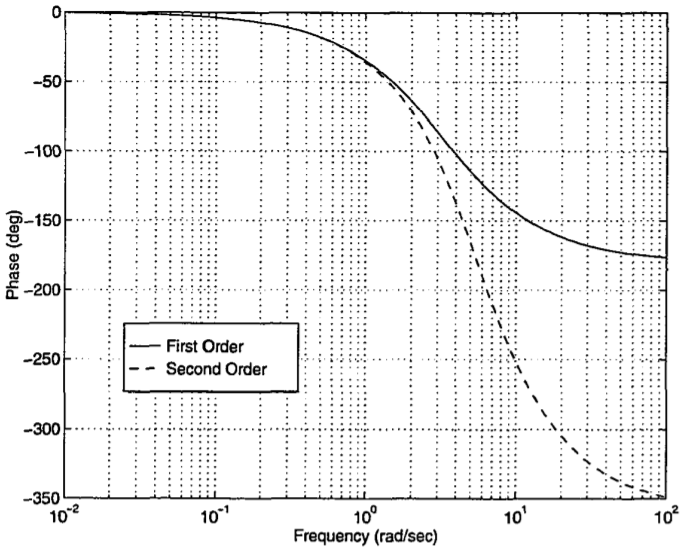
\includegraphics[scale = .6]{Figure 4.1}
	\bf\caption{ Phase lag from the Fad\'{e} approximations o f time delay.}
	\label{fig:4.1}
\end{figure}

\begin{figure}[H]
	\centering
	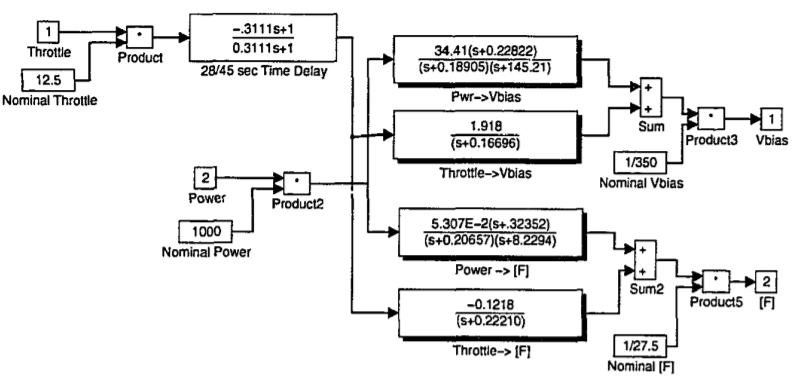
\includegraphics[scale = .6]{Figure 4.2}
	\bf\caption{ Simulink block diagram: plasma generation process model.}
	\label{fig:4.2}
\end{figure}

\noindent the Simulink command linmod [73] was used to create the state space representation

\begin{align*}
	\dot x(t) = A_{p} x(t) + B_{p}u(t)
\end{align*}

\begin{align}
	y(t) = C_{p} x(t) + D_{p}u(t)
\end{align}

\noindent where $u(t)$ are the process inputs, $y(t)$ are the process outputs, $x(t)$ are the states of the model, and

\begin{align}
	\renewcommand\arraystretch{2} A_{p} &= \begin{bmatrix}
		-8.436 & -1.304 & 0 & 0 & 0 & 0 & 0 \\ 1.304 & 0 & 0 & 0 & 0 & 0 & 0 \\ 0 & 0 & -0.2221 & 0 & 0 & 0 & 6.429 \\ 0 & 0 & 0 & -145.4 & -5.239 & 0 & 0 \\ 0 & 0 & 0 & 5.239 & 0 & 0 & 0 \\ 0 & 0 & 0 & 0 & 0 & -0.167 & 6.429 \\ 0 & 0 & 0 & 0 & 0 & 0 & -3.214 
	\end{bmatrix} \\
	B_{p} &= \begin{bmatrix}
		0 & 1000 \\ 0 & 0 \\ -12.5 & 0 \\ 0 & 1000 \\ 0 & 0 \\ -12.5 & 0 \\ 12.5 & 0
	\end{bmatrix} \\
	C_{p} &= \begin{bmatrix}
		0 & 0 & 0 & 0.0983 & 0.0043 & 0.0055 & 0 \\ 0.0019 & 0.0005 & -0.0044 & 0 & 0 & 0 & 0
	\end{bmatrix} \\
	D_{p} &= \begin{bmatrix}
		0 & 0 \\ 0 & 0
	\end{bmatrix}
\end{align}

\setstretch{1.5}
\noindent This model of the system dynamics is known as the p la n t For the rest of this dissertation, the time dependence will be dropped from this notation and it should be understood that the inputs $u$, states $x$ , and outputs $y$ are all functions of time. Also, since $D_{p}=0$, it does not enter into the calculations presented below.


The most important performance objective was to have zero steady-state error in tracking plasma setpoints. This was accomplished by using integral control [25]. The first step in the design was to augment the system with integrators. A set of states $q$, equal to the integral of the error between the plant output and the desired output $r$, was defined by

\setstretch{1}
\begin{align}
	\dot q = y-r.
\end{align}

\noindent Augmenting the system in Equation 4.2 with these states, the new plant became

\begin{align*}
	\begin{bmatrix}
		\dot x \\ \dot q
	\end{bmatrix} &=
	\myunderbrace{\begin{bmatrix}
			A_{p} & 0 \\ C_{p} & 0 
	\end{bmatrix}}{A_{m}} 
	\begin{bmatrix}
		x \\ q
	\end{bmatrix} + 
	\myunderbrace{\begin{bmatrix}
			B_{p} \\ 0
	\end{bmatrix}}{B_{m}} u +
	\myunderbrace{\begin{bmatrix}
			0 \\ -I
	\end{bmatrix}}{G_{m}} r,
\end{align*}

\begin{align}
	y &= 
	\myunderbrace{\begin{bmatrix}
			C_{p} & 0 
	\end{bmatrix}}{C_{m}} 
	\begin{bmatrix} 
		x \\ q
	\end{bmatrix}.
\end{align}

\noindent To simplify notation, we define the augmented state vector $ x_{m} = \begin{bmatrix}
	x \\ q
\end{bmatrix}$ and rewrite Equation 4.8 as

\begin{align*}
	\dot x = A_{m}x_{m} + B_{m}u + G_{m} r
\end{align*}

\begin{align}
	y = C_{m} x_{m} . 
\end{align}

\begin{figure}[H]
	\centering
	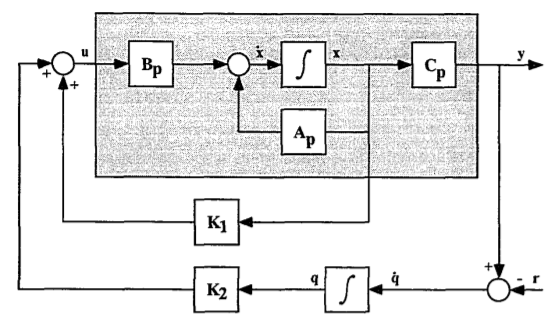
\includegraphics[scale = .75]{Figure 4.3}
	\bf\caption{ State feedback diagram.}
	\label{fig:4.3}
\end{figure}

\setstretch{1.5}
In selecting the feedback gains, it was first assumed that the states $x_{m}$ were measurable and that the controlled inputs had the form


\setstretch{1}
\begin{align}
	u = -Kx_{m},
\end{align}

\noindent where

\begin{align}
	K = \begin{bmatrix}
		K_{1} & K_{2}
	\end{bmatrix}
\end{align}

\setstretch{1.5}
was the state feedback gain as shown in Figure 4.3. This state feedback gain was found by solving the linear quadratic regulator (LQR) problem. Briefly, in the LQR problem the controller gain $K$ is found by minimizing the cost function


\setstretch{1}
\begin{align}
	J = \int_{0}^{\infty} \left( x'Qx+u'Ru \right) dt,
\end{align}

\setstretch{1.5}
subject to the system in Equation 4.9 and the control input from Equation 4.10. In this equation, $Q$ is a matrix of weights for the states and $R$ is a matrix of weights for the inputs. Complete details of the LQR problem can be found in [4]. In this research, the weight
matrix for the states had the form

\setstretch{1}
\begin{align}
	\renewcommand\arraystretch{1.5} Q = \begin{bmatrix}
		\alpha C'_{p}C_{p} & 0 \\ 0 & Q_{p}
	\end{bmatrix}
\end{align}

\setstretch{1.5}
\noindent where $\alpha$ was a scalar and $Q_{q}$ was a diagonal matrix of the weights for each integrator state. The input weight matrix $R$ was a diagonal matrix of weights for each individual input.

Applying the control inputs from Equation 4.10 to the system in Equation 4.9 yields the following closed loop system


\setstretch{1}
\begin{align*}
	\dot x_{m} = \left( A_{m} - B_{m}K \right) x_{m} + G_{m} r
\end{align*}

\begin{align}
	y = C_{m}x_{m}.
\end{align}

\setstretch{1.5}
\noindent Parameters for the weight matrices were chosen and the closed loop system simulated to determine if the performance objectives and design constraints were satisfied. After several iterations, the following parameters were settled upon

\setstretch{1}
\begin{align}
	\alpha &= 1,\\
	Q_{p} &= \begin{bmatrix}
		0.6 & 0.0 \\ 0.0 & 0.5 
	\end{bmatrix},
\end{align}

\noindent and

\begin{align}
	R = \begin{bmatrix}
		4.0 & 0.0 \\ 0.0 & 3.0 
	\end{bmatrix}.
\end{align}

\setstretch{1.5}
\noindent The Iqr command from the Matlab Control Systems Toolbox [40] was used to calculate the state feedback gains

\setstretch{1}
\begin{align}
	\renewcommand\arraystretch{1.5}
	K_{1} = \begin{bmatrix}
		0.000 & 0.000 & 0.006 & 0.000 & 0.001 & 0.004 & 0.019 \\ 0.000 & 0.000 & -0.002 & 0.011 & 0.001 & 0.005 & 0.004
	\end{bmatrix}
\end{align}

\begin{figure}[H]
	\centering
	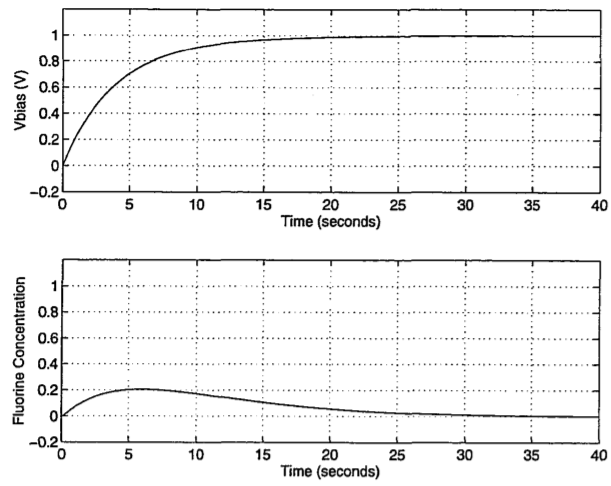
\includegraphics[scale = .6]{Figure 4.4}
	\bf\caption{ Simulated response of closed loop system to a step in $\text{V}_{bias}$}
	\label{fig:4.4}
\end{figure}

\noindent and

\begin{align}
	K_{2} = \begin{bmatrix}
		0.162 & -0.321 \\ 0.406 & 0.171
	\end{bmatrix}.
\end{align}

\setstretch{1.5}
\noindent Figure 4.4 shows the simulated response of the plasma to a step change in the $\text{V}_{bias}$ command. The corresponding responses of the actuators are shown in Figure 4.5. Likewise, the plasma and actuator responses for a step change in the fluorine concentration setpoint are shown in Figures 4.6 and 4.7.

\noindent\textbf{Observer Design}

In practice, the states of the system are not available for feedback, therefore they must be estimated. Actually, only the states of the plant $x$ needed to be estimated, as the integrated error states $q$ are calculated in the controller. The true system has disturbances

\setstretch{1}
\begin{figure}[H]
	\centering
	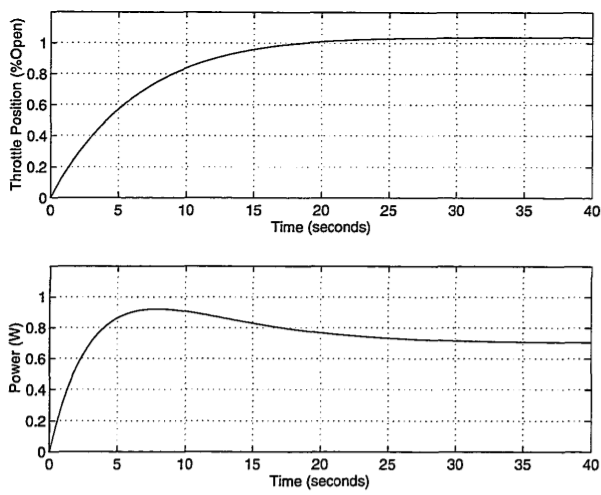
\includegraphics[scale = .6]{Figure 4.5}
	\bf\caption{ Simulated response of actuators to a step in $\text{V}_{bias}$.}
	\label{fig:4.5}
\end{figure}

\begin{figure}[H]
	\centering
	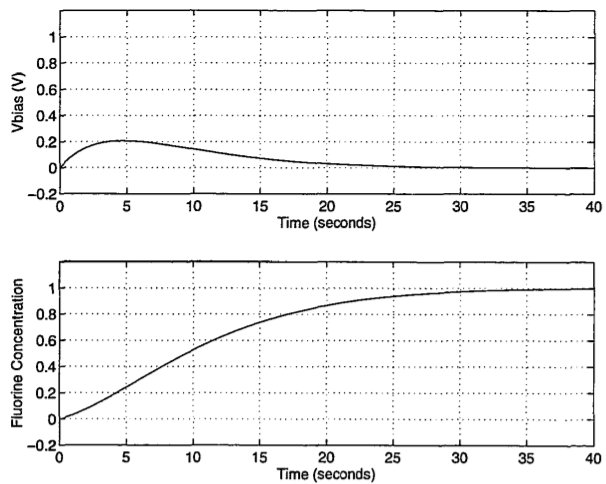
\includegraphics[scale = .6]{Figure 4.6}
	\bf\caption{ Simulated response of closed loop system to a step in fluorine concentration.
	}
	\label{fig:4.6}
\end{figure}

\begin{figure}[H]
	\centering
	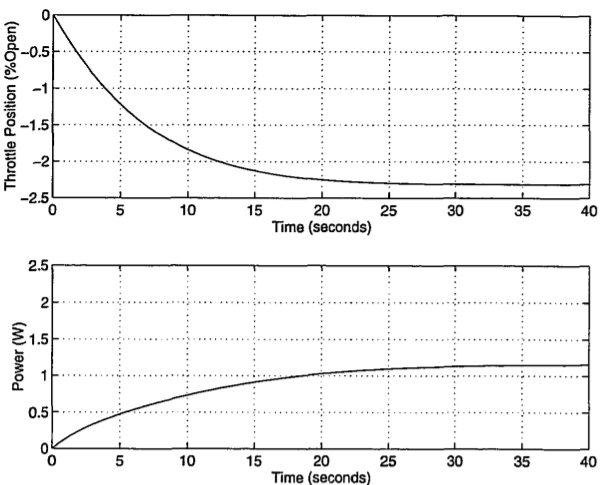
\includegraphics[scale = .75]{Figure 4.7}
	\bf\caption{ Simulated response of actuators to a step in fluorine concentration.}
	\label{fig:4.7}
\end{figure}

to the process and noise in the measurements. This was represented by

\begin{align*}
	\dot x(t) = A_{p}x+B_{p}u+v
\end{align*}

\begin{align}
	y(t) = C_{p}x+w,
\end{align}

\setstretch{1.5}
where $v$ and $w$ were assumed to be white noise. The states of this system were then estimated using an observer of the form [17]


\setstretch{1}
\begin{align}
	\dot{\hat{x}} = A_{p}x + B_{p}u + L'(y-\hat{y}),
\end{align}

\setstretch{1.5}
\noindent where $L'$ is the observer gain and $\hat{y} = C_{p}\hat{x}$. The LQG/LTR technique [26] was used to find the observer gain by minimizing the the covariance between the actual and estimated values for the states. The lqr command was used again to find this gain. However, this time the LQR problem was solved for ($A'_{p}$,$C'_{p}$) where the weightings were the covariance matrices $V$ and $W$ , for the process and measurement noise, respectively. These matrices were assumed to have the following form


\setstretch{1}
\begin{align}
	V = B'_{p} B_{p}
\end{align}

and

\begin{align}
	W = \rho I,
\end{align}

\setstretch{1.5} 
\noindent where $I$ is the identity matrix and $\rho$ is a scalar. For the PGP controller $\rho = 1$ was used.

Combining the observer with the state feedback gain leads to a controller of the form

\setstretch{1}
\begin{align*}
	\renewcommand\arraystretch{1.5}
	\begin{bmatrix}
		\dot{\hat{x}} \\ \dot q
	\end{bmatrix} &=
	\myunderbrace{\begin{bmatrix}
			A_{p}-B_{p}K_{1}-L'C_{p} & -B_{p}K_{2} \\ 0 & 0 
	\end{bmatrix}}{A_{c}} 
	\begin{bmatrix}
		\hat{x} \\ q
	\end{bmatrix} + 
	\myunderbrace{\begin{bmatrix}
			L' & 0 \\ I & -I
	\end{bmatrix}}{B_{b}} +
	\begin{bmatrix}
		y \\ r
	\end{bmatrix}
\end{align*}

\begin{align}
	\renewcommand\arraystretch{2}
	u = \myunderbrace{-K}{C_{c}} \begin{bmatrix}
		\hat{x} \\ q 
	\end{bmatrix}.
\end{align}

\begin{figure}[H]
	\centering
	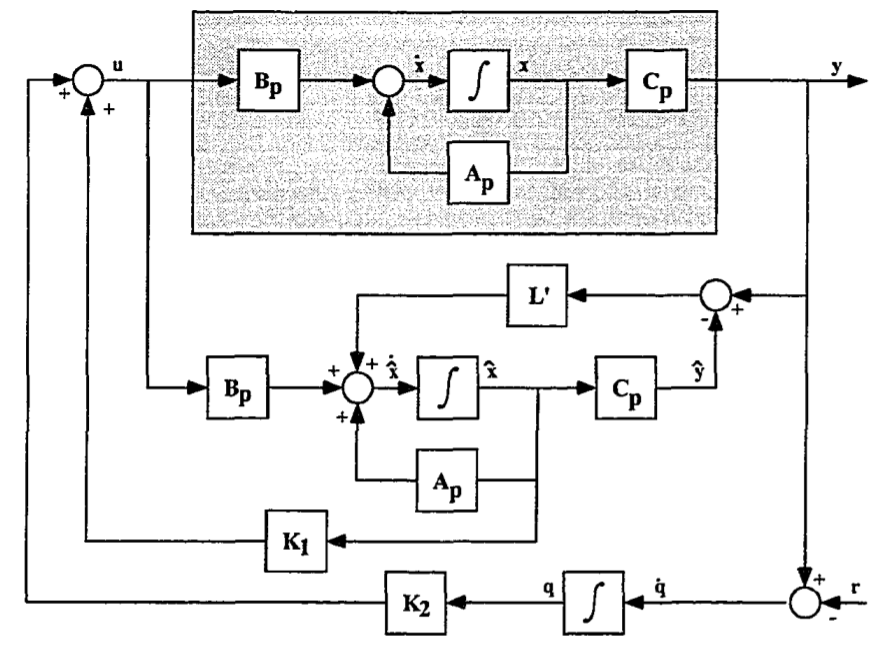
\includegraphics[scale = .5]{Figure 4.8}
	\bf\caption{ LQG/LTR closed loop system.}
	\label{fig:4.8}
\end{figure}

\noindent Defining the controller states as $x_{c}=\begin{bmatrix}
	\hat{x} \\ q
\end{bmatrix}$ yields the closed loop system

\begin{align*}
	\renewcommand\arraystretch{1.5}
	\begin{bmatrix}
		\dot x_{c} \\ \dot{x}
	\end{bmatrix} = 
	\begin{bmatrix}
		A_{c} & B_{c}C_{p} \\ B_{p}C_{c} & A_{p}
	\end{bmatrix}
	\begin{bmatrix}
		x_{c} \\ x
	\end{bmatrix} +
	\begin{bmatrix}
		0 \\ -I
	\end{bmatrix} r,
\end{align*}

\begin{align}
	\renewcommand\arraystretch{1.5}
	y = \begin{bmatrix}
		0 &  C_{p} 
	\end{bmatrix}
	\begin{bmatrix}
		x_{c} \\ x
	\end{bmatrix}.
\end{align}

\setstretch{1.5}
\noindent The closed loop system is shown graphically in Figure 4.8. Simulations showed that this controller had virtually identical performance to the state feedback design.

\noindent\textbf{Model Reduction}

In order to reduce the computational complexity of the controller, states that weakly affect the input-output properties were eliminated. This is known as \textit{model order reduction} and was done using a technique called balanced truncation. The states of the controller were transformed from physically meaningful variables to a balanced realization. In this realization the relative effect of each state on the input-output dynamics of the controller can be examined. Details of this method of model reduction can be found in [60].

In order to transform the controller into a balanced realization, the integrator states must first be removed. The controller was therefore decomposed into two parts

\setstretch{1}
\begin{align*}
	\renewcommand\arraystretch{1.5}
	\begin{bmatrix}
		\dot{q}
	\end{bmatrix} = 
	\myunderbrace{\begin{bmatrix}
			0
	\end{bmatrix}}{A_{i}}
	\begin{bmatrix}
		q
	\end{bmatrix} +
	\myunderbrace{\begin{bmatrix}
			I & -I 
	\end{bmatrix}}{B_{i}}
	\begin{bmatrix}
		y \\ r
	\end{bmatrix}
\end{align*}

\begin{align}
	\renewcommand\arraystretch{1.5}
	\begin{bmatrix}
		u_{q} \\ y
	\end{bmatrix}
	\myunderbrace{\begin{bmatrix}
			-K_{2} \\ 0 
	\end{bmatrix}}{C_{i}} 
	\begin{bmatrix}
		q
	\end{bmatrix} +
	\myunderbrace{\begin{bmatrix}
			0 & 0 \\ I & 0
	\end{bmatrix}}{D_{i}}
	\begin{bmatrix}
		y \\ r
	\end{bmatrix}
\end{align}

\noindent and

\begin{align*}
	\renewcommand\arraystretch{1.5}
	\begin{bmatrix}
		\dot{\hat{x}}
	\end{bmatrix} = 
	\myunderbrace{\begin{bmatrix}
			A_{p}-B_{p}K_{1}-L'C_{p}
	\end{bmatrix}}{A_{s}}
	\begin{bmatrix}
		\hat{x}
	\end{bmatrix} + 
	\myunderbrace{\begin{bmatrix}
			B_{p} & L' 
	\end{bmatrix}}{B_{s}}
	\begin{bmatrix}
		u_{q} \\ y
	\end{bmatrix}
\end{align*}

\begin{align}
	\renewcommand\arraystretch{1.5}
	u = 
	\myunderbrace{\begin{bmatrix}
			-K_{1}
	\end{bmatrix}}{C_{s}} \hat{x} +
	\myunderbrace{\begin{bmatrix}
			I & 0
	\end{bmatrix}}{D_{s}}
	\begin{bmatrix}
		u_{q} \\ y
	\end{bmatrix}
\end{align}

\setstretch{1.5}
\noindent where the system [$A_{i},B_{i},C_{i},D_{i}$] was the integral portion and the system [$A_{s},B_{s},C_{s},D_{s}$] was the state feedback portion. The state feedback portion was then balanced using the balreal command from the Matlab Control System Toolbox. From this command, the relative effect of each state on the input-output dynamics was found to be


\setstretch{1}
\begin{align}
	g = \begin{bmatrix}
		0.2119 & 0.0610 & 0.0313 & 0.0045 & 0.0036 & 0.0006 & 0.0001
	\end{bmatrix}.
\end{align}

\setstretch{1.5}
\noindent The order of the controller was then reduced by eliminating those states corresponding to elements of g more than an order of magnitude smaller than the largest element. This was done using the m o d re d command and yielded a reduced state feedback portion with three states. Incorporating the integral states back into the controller yielded

\setstretch{1}
\begin{align}
	A_{cr} &= \renewcommand\arraystretch{1.25}\begin{bmatrix}
		-0.3297 & 0.0269 & -0.4947 & -0.0545 & 0.1201 \\ -0.1154 & -2.1648 & 14.9135 & 0.1731 & 0.0997 \\ 0.7559 & 14.7504 & -114.6750 & -0.9359 & -0.5572 \\ 0 & 0 & 0 & 0 & 0 \\ 0 & 0 & 0 & 0 & 0
	\end{bmatrix} \\
	B_{cr} &= \renewcommand\arraystretch{1.25}\begin{bmatrix}
		0.0465 & -0.0494 & 0 & 0 \\ -0.2259 & -0.0478 & 0 & 0 \\ 0.9371 & 0.0661 & 0 & 0 \\ 1.0000 & 0 & -1.0000 & 0 \\ 0 & 1.0000 & 0 & -1.0000
	\end{bmatrix} \\
	C_{cr} &= \renewcommand\arraystretch{1.25}\begin{bmatrix}
		-0.3637 & -0.1224 & 0.4062 & -0.1612 & 0.3234 \\ -0.0865 & 0.4990 & -2.6466 & -0.4024 & -0.1707
	\end{bmatrix} \\
	D_{cr} &= \renewcommand\arraystretch{1.25}\begin{bmatrix}
		-0.0000345 & 0.0003689 & 0 & 0 \\ -0.0005203 & 0.0003663 & 0 & 0
	\end{bmatrix}
\end{align}

\setstretch{1.5}
\noindent The Bode plots of the gains of the full and reduced order controllers from $\text{V}_{bias}$ and fluorine concentration are shown in Figures 4.9 and 4.10, respectively. As can be clearly seen, the reduced order controller has very similar input-output properties to the full order controller.

\setstretch{1}
\begin{figure}[H]
	\centering
	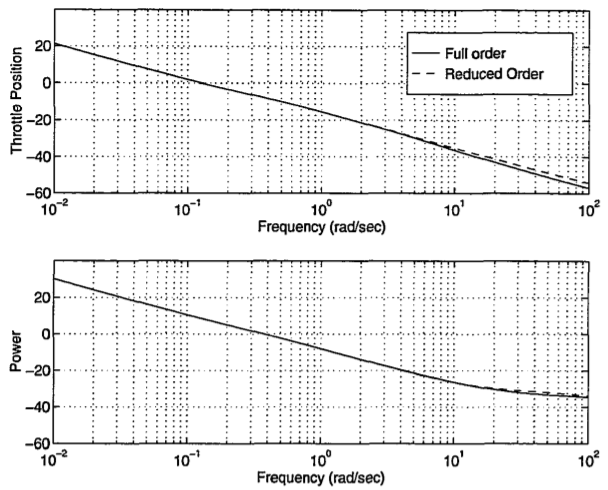
\includegraphics[scale = 0.5]{Figure 4.9}
	\bf\caption{ Controller gains from $\text{V}_{bias}.$}
	\label{fig:4.9}
\end{figure}

\begin{figure}[H]
	\centering
	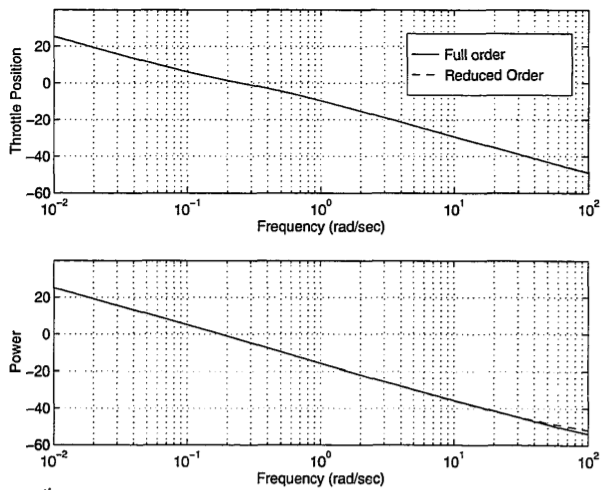
\includegraphics[scale = .5]{Figure 4.10}
	\bf\caption{ Controller gains from fluorine concentration.}
	\label{fig:4.10}
\end{figure}

\setstretch{1.5}
\subsection{Implementation}

\tab The controller design was based on a model of the PG P with normalized inputs and
outputs. Before the controller could be implemented, these scalings need to be incorporated.
This was done in the Simulink block diagram shown in Figure 4.11. Also, the controller
needed to be discretized for implementation on a digital computer (using the Lab VIEW
system described in Section 2.2). This was accomplished using the c2d command from the
Matlab Control Systems Toolbox and yielded a controller of the structure


\setstretch{1}
\begin{align*}
	x(k+1) = \bar{A}_{c}x(k) + \bar{B}_{c} \renewcommand\arraystretch{1.5}\begin{bmatrix}
		y(k) \\ r(k)
	\end{bmatrix},
\end{align*}

\begin{align}
	u(k+1) = \bar{C}_{c}x(k) + \bar{D}_{c} \renewcommand\arraystretch{1.5}\begin{bmatrix}
		y(k) \\ r(k)
	\end{bmatrix}.
\end{align}

\setstretch{1.5}
\section{Disturbance Rejection Experiments}

\tab A number of experiments were designed to examine the ability of the plasma generation
process controller to attenuate process disturbances. The controller was compared to the
standard practice in.its ability to reject disturbances to etch rate. Etches were performed
on unmasked wafers with material layers polysilicon/$\text{SiO}_{2}$/Si substrate. Etch rate data was collected in real time using the reflectometry system described in Section 2.1.4. This data was processed after the experiments, as described in Section 2.1.4, and was not available to be used for etch rate control.

\begin{figure}[H]
	\centering
	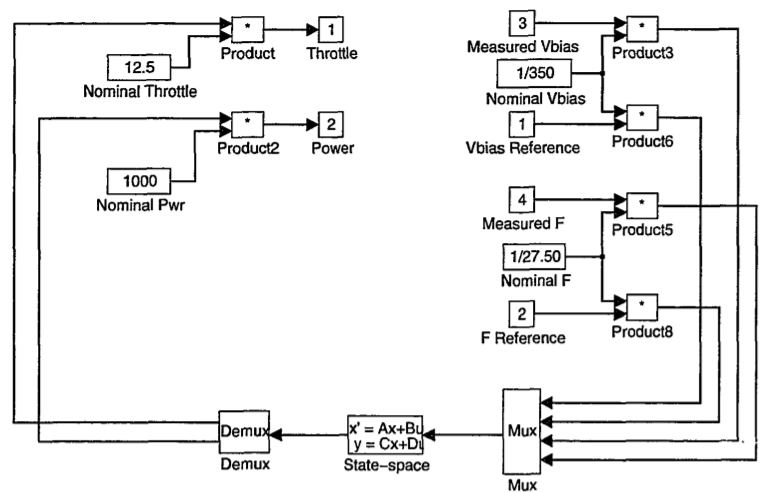
\includegraphics[scale = .75]{Figure 4.11}
	\bf\caption{ Simulink block diagram: controller structure.}
	\label{fig:4.11}
\end{figure}

\subsection{Description of Experiments}
\tab All of the experiments have a common disturbance due to the lack of a load lock on our
AME-8300. W ithout a load lock, the chamber must be opened to the ambient atmosphere
when a wafer is loaded before each etch. As a result, water vapor adsorbs onto the inner
walls of the reactor; the thickness of this film seems to vary with the degree of polymer
buildup on the reactor’s inner surfaces and the ambient conditions in the cleanroom. The
desorption of this moisture into the chamber acts as a “wall disturbance” to the etch process
and is present in all of our experiments. As our reactor has a large surface area, this is a
very large disturbance. While in a production environment etchers are usually load locked,
the condition of the chamber walls varies as the reactor seasons. We shall use the wall
disturbance as a test to demonstrate the power of feedback control.

The experiments that were run are now described:

\begin{enumerate}
	\item \textit{Baseline, Standard Practice Etch:} This etch was run with the pressure, $\text{CF}_{4}$ flow rate, and applied power set to their nominal values, i.e., 20 mTorr, 30 sccm, and 1000 W, respectively. In this experiment, pressure was regulated by a PID loop internal to the throttle valve controller, and $\text{V}_{bias}$ and $[F]$ were not regulated.
	
	\item \textit{Baseline, Closed-Loop Etch:} In this case, the plasma generation process controller was used to demonstrate the efficacy of feedback control in reducing the effect of the wall disturbance upon etch rate. The setpoints for $\text{V}_{bias}$ and $[F]$ were chosen to be 342 V and 47.1 (arbitrary units), respectively.
	\item \textit{Loading Effect Experiment:} The amount of exposed surface area to be etched will often vary from batch to batch or during a single run as material is removed; see Figure 4.12. As the amount of exposed material on the wafer increases, so does the
	\begin{figure}[H]
		\centering
		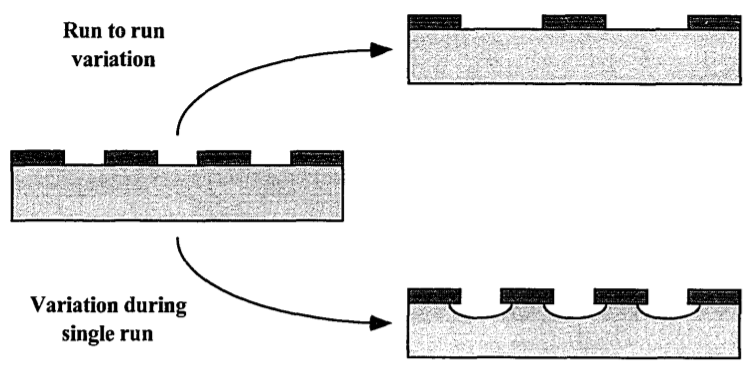
\includegraphics[scale = .5]{Figure 4.12}
		\bf\caption{ Loading effect.}
		\label{fig:4.12}
	\end{figure}
	rate of consumption of the etchant. This may result in a decrease in the etch rate,
	and is often referred to as the “loading effect” [109]. To assess the effect of a loading
	disturbance upon etch rate, etches were run with two wafers in the chamber, instead
	of just one, therefore doubling the area of exposed silicon.
	\item \textit{Oxygen Leak Experiment:} The addition of small amounts of oxygen has been found empirically to cause a significant increase in the etch rate of polysilicon. It is believed that this is caused by reactions between $\text{CF}_{x},x=(1-3)$, and oxygen atoms. These reactions liberate more fluorine atoms and prevent recombination, thus resulting in an increased fluorine concentration [85]. The effect of an $\text{O}_{2}$ disturbance on etch rate was explored by introducing 1 sccm of $\text{O}_{2}$ in increments of $\frac{1}{2}$ sccm of $\text{O}_{2}$ applied at 600 and 1200 seconds into the etch.
	
	\item \textit{Power Mismatch Experiment:} As mentioned previously, an rf matching network was used for impedance matching between the power source and the reactor load. The impact of variations in the matching network or other variations in the power supply
	was examined by having the power generation unit respond with 2\% more power
	\begin{figure}[H]
		\centering
		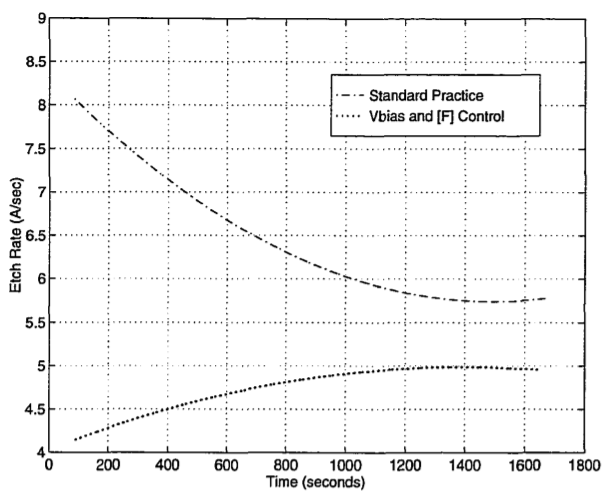
\includegraphics[scale = .5]{Figure 4.13}
		\bf\caption{ Wall disturbance experiment.}
		\label{fig:4.13}
	\end{figure}
	than was commanded. In the open-loop case, this resulted in shifting the power from
	lOOOW to 1020W.
\end{enumerate}

\noindent In all of the experiments the wall disturbance was present. Therefore, the first two experiments serve as a baseline to which the others were compared.

\subsection{Experimental Results}

\tab In Figure 4.13, the dash-dot curve is the etch rate under a standard practice open-loop
etch. Notice that the etch rate decreased slowly over the length of the experiment. As
can be seen in Figure 4.14, the fluorine concentration follows a similar trajectory during the etch. A possible explanation for this is that, during the initial phase of the etch, a significant amount of moisture is desorbed from the walls into the chamber. This moisture leads to an increased fluorine concentration and hence increased etch rate[84]. This hypothesis is supported by experiments that showed that optical emission from the 451.1 nm line of CO
followed a trajectory similar to that of fluorine concentration. As the experiment progresses, the desorption of moisture decreases, as does the etch rate. The etch rate under the closedloop conditions is shown by the dotted hue. The corresponse trajectories for the plasma characteristics and actuator commands are shown in Figure 4.15 and 4.16, respectively. As one can see, the etch rate was much more constant under closed-loop conditions. The etch rates settled to different values because the setpoints under closed-loop control were different from the steady-state values of the plasma conditions in the open-loop experiment\footnote{The reason that the plasma setpoints did not match the open-loop steady-state values was due to operator error.}. In Figure 4.17 it is shown that, if the plasma setpoints are chosen to be the steady-state open-loop conditions, then the etch rates do indeed settle to the same rate. 

In this closed-loop experiment, as well as the others, the etch rate started off below the steadystate value. However, the values of $\text{V}_{bias}$ and $[F]$ remain constant throughout the etch. One potential explanation is th at the fluorine estimate, $[F]=\frac{I_{F}}{I_{Ar}}P$ , overestimated the fluorine concentration resulting from the Og disturbance [47]. The controller responded by reducing the actual fluorine concentration below the desired value and thus decreased the etch rate. As the disturbance decayed during the run, the estimate was more accurate and the etch rate approached its steady-state value. Another possible reason for the reduced etch rate during the first portion of the etch is that factors other than $\text{V}_{bias}$ and $[F]$ affect the etch rate. In other words, while regulating $\text{V}_{bias}$ and $[F]$ does reduce the impact of the disturbance substantially, it does not eliminate its effect.


Figure 4.18 shows the etch rates during the loading effect experiment. Here, the dashed
curve represents the open-loop etch rate while the solid curve represents the closed-loop etch rate. The dash-dot and dotted lines from the wall disturbance experiments are included on this and the other plots to make comparisons easier. 


\setstretch{1}
\begin{figure}[H]
	\centering
	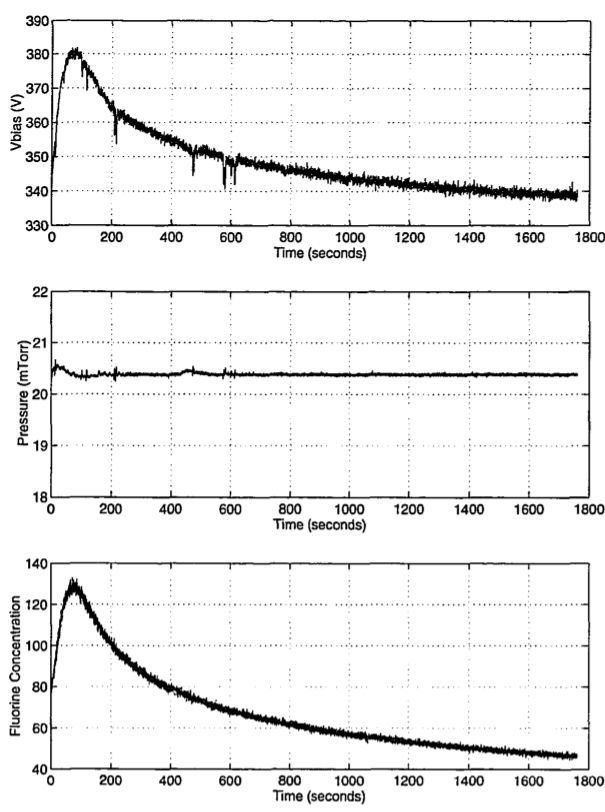
\includegraphics[scale = .75]{Figure 4.14}
	\bf\caption{  Response of plasma characteristics during standard practice etch.}
	\label{fig:4.14}
\end{figure}

\begin{figure}[H]
	\centering
	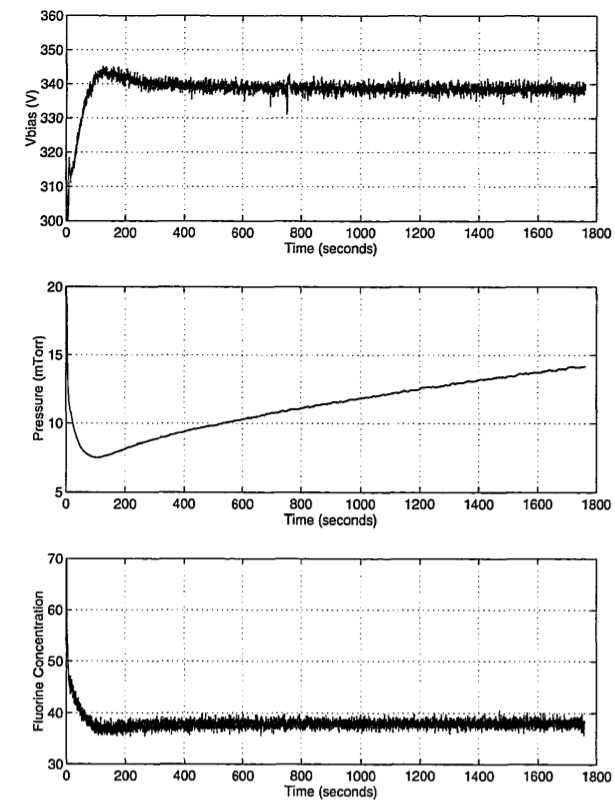
\includegraphics[scale = .75]{Figure 4.15}
	\bf\caption{  Response of plasma characteristics during closed-loop etch.}
	\label{fig:4.15}
\end{figure}

\begin{figure}[H]
	\centering
	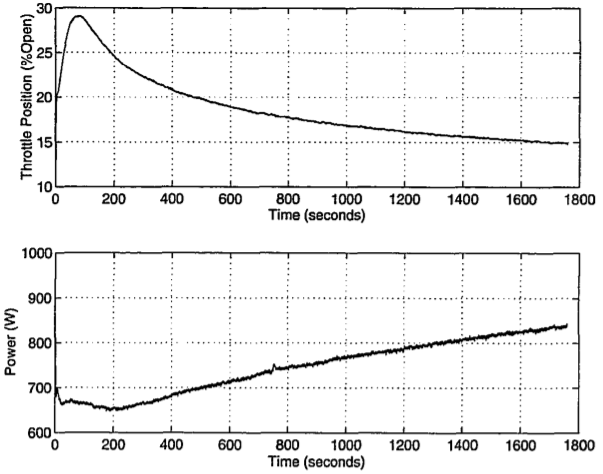
\includegraphics[scale = .6]{Figure 4.16}
	\bf\caption{  Corresponding actuator responses during closed-loop etch.}
	\label{fig:4.16}
\end{figure}

\begin{figure}[H]
	\centering
	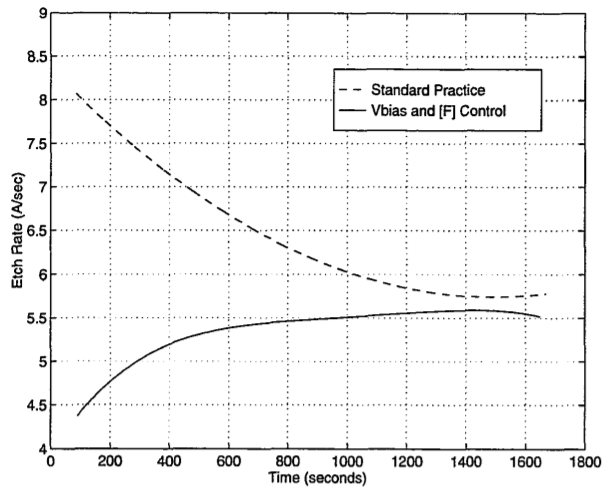
\includegraphics[scale = .6]{Figure 4.17}
	\bf\caption{  Etch rate with plasma setpoints matching steady-state conditions from standard practice baseline etch.}
	\label{fig:4.17}
\end{figure}

\begin{figure}[H]
	\centering
	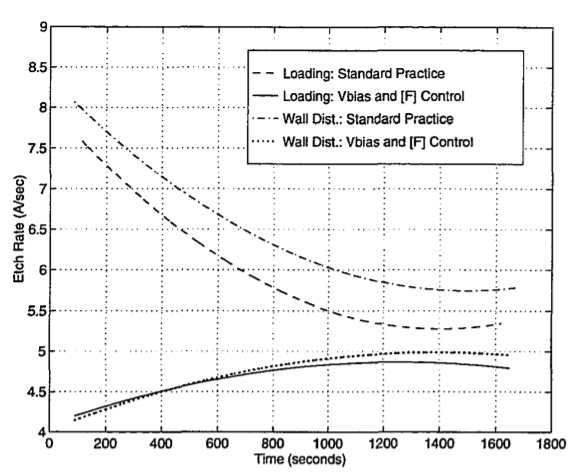
\includegraphics[scale = .5]{Figure 4.18}
	\bf\caption{  Loading experiment.}
	\label{fig:4.18}
\end{figure}

\setstretch{1.5}
\noindent As expected, increased loading led to a decrease in etch rate under open-loop conditions. However, comparison of the closed-loop data (the solid and dotted lines) showed that the impact of the loading on etch rate was greatly attenuated.

Etch rate data for the oxygen leak experiment is shown in Figure 4.19. Notice that upon
injection of oxygen, the etch rate increased during the standard practice etch, as expected.
Under closed-loop conditions, the addition of oxygen appeared to make virtually no difference to the etch rate. However, recall from Section 2.1.4 that the etch rate measurement was
actually the average rate between a peak and valley in the reflected interference pattern.
During the disturbance experiments, etch rate measurements were available approximately
every 90 seconds. Therefore, it is likely that the etch rate did change at each step in $\text{O}_{2}$ flow, but the effect was attenuated before the next etch rate measurement was available. Notice that, despite very similar operating conditions, there was a difference in the openloop experiment between the dashed curve and the dash-dot curve even before the injection of oxygen. An explanation for this phenomenon is that the amount of moisture absorbed on the walls varies from

\setstretch{1}
\begin{figure}[H]
	\centering
	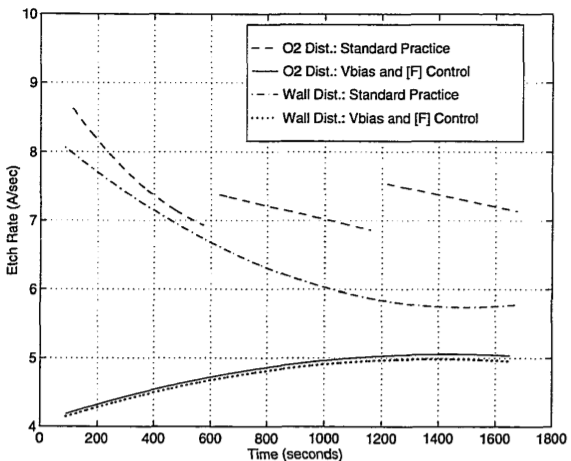
\includegraphics[scale = .55]{Figure 4.19}
	\bf\caption{  Oxygen disturbance experiment.}
	\label{fig:4.19}
\end{figure}

\setstretch{1.5}
\noindent etch to etch depending upon the duration of the exposure to the
atmosphere while loading the wafer and the condition of the chamber.

Finally, the power disturbance results are shown in Figure 4.20. As expected, an increase
in applied power increased the etch rate under open-loop conditions. However, under closedloop control, there was a much smaller change in etch rate.

These results demonstrate that closed-loop control of the key plasma parameters, such
as $\text{V}_{bias}$ and $[F]$, can result in a significant reduction in the effects of common disturbances as compared to the standard practice open-loop etches. This was certainly quite true for the loading effects, oxygen disturbance, and the power disturbance. This can be seen very clearly in Figure 4.21, where results from the various disturbances using each control strategy are presented again. Even for the wall disturbance, we have achieved a significant reduction in the impact of the disturbance, but there is room for improvement.

\setstretch{1}
\begin{figure}[H]
	\centering
	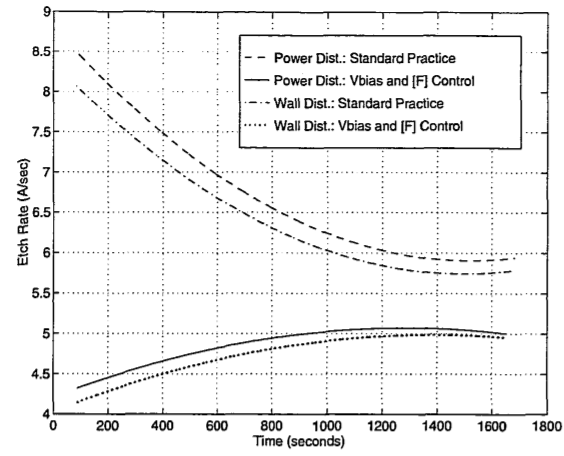
\includegraphics[scale = .55]{Figure 4.20}
	\bf\caption{  Power disturbance experiment.}
	\label{fig:4.20}
\end{figure}

\setstretch{1.5}
\section{Comparison of Vbias/[F] vs. Vbias/Pressure Control}

\tab It is becoming common in industrial applications to use feedback control to regulate
both pressure and $\text{V}_{bias}$. The oxygen disturbance experiment was repeated to compare the effect of controlling only pressure, $\text{V}_{bias}$ and pressure, and $\text{V}_{bias}$ and fluorine concentration. In this experiment, 1 sccm of $\text{O}_{2}$ was introduced into the feed gas at 600 seconds into the etch. As can be seen in Figure 4.22, that while $\text{V}_{bias}$/pressure control slightly attenuates the effect of the wall disturbance during the first portion of the etch, this strategy is ineffective against the oxygen disturbance. This result is not surprising as the oxygen disturbance primarily effects etch chemistry and hence fluorine concentration.


\setstretch{1}
\begin{figure}[H]
	\centering
	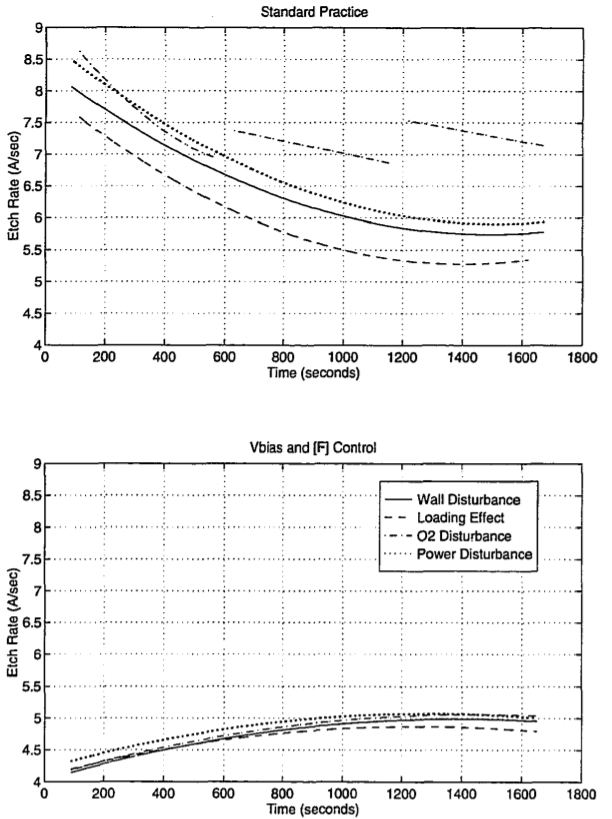
\includegraphics[scale = .75]{Figure 4.21}
	\bf\caption{  Comparison of the effects of the various disturbances.}
	\label{fig:4.21}
\end{figure}

\begin{figure}[H]
	\centering
	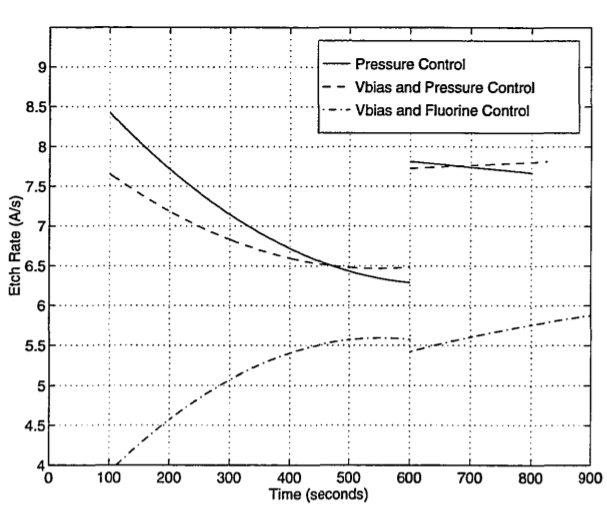
\includegraphics[scale = .75]{Figure 4.22}
	\bf\caption{  Comparison of controlling pressure, $\text{V}_{bias}$/pressure, and $\text{V}_{bias}$/[Fp}
	\label{fig:4.22}
\end{figure}
